\chapter{Joshua 17}

\begin{figure}
  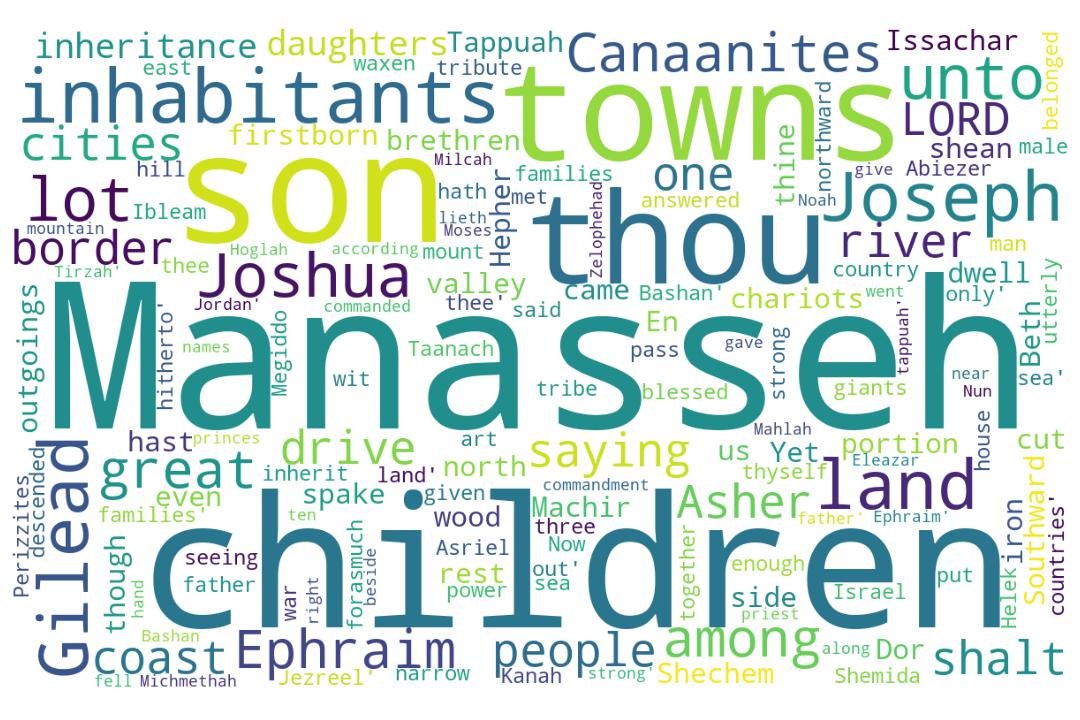
\includegraphics[width=\linewidth]{06OT-Joshua/Joshua17-WordCloud.jpg}
  \caption{Joshua 17 Word Cloud}
  \label{fig:Joshua 17 Word Cloud}
\end{figure}

\marginpar{\scriptsize \centering \fcolorbox{bone}{lime}{\textbf{MANASSEH ON THE WEST SIDE}}\\ (Joshua 17:1-18) \begin{compactenum}[I.][8]
	\item The \textbf{Daughters}  \index[scripture]{Joshua!Jsh 16:03}\index[scripture]{Joshua!Jsh 17:06}  (Jsh 17:3, 6) 
	\item The \textbf{Decree}  \index[scripture]{Joshua!Jsh 16:04}  (Joshua 17:4) (so what happens when the male line to the throne is cut off? This decree determines that Mary's descendant has a right to the throne
	\item The \textbf{Descendants} (the word ``children'' found 13 times in the chapter\index[scripture]{Joshua!Jsh 16:02}  \index[scripture]{Joshua!Jsh 17:08}  \index[scripture]{Joshua!Jsh 17:13}  \index[scripture]{Joshua!Jsh 17:14}  \index[scripture]{Joshua!Jsh 17:16}  (Jsh 17:2 (8x), 8, 12, 13, 14, 16) 
	\item The \textbf{Dwellers}  \index[scripture]{Joshua!Jsh 17:12}\index[scripture]{Joshua!Jsh 17:16}   (Joshua Jsh:12, 16) 
	\item \textbf{Drive} out the Canaanites \index[scripture]{Joshua!Jsh 17:12}\index[scripture]{Joshua!Jsh 17:13} \index[scripture]{Joshua!Jsh 17:18}  (Jsh 17:12, 13, 18) 
	\item We're \textbf{Disdavantaged}  \index[scripture]{Joshua!Jsh 17:12}\index[scripture]{Joshua!Jsh 17:16}   (Jsh 17:16) 
	\item Joshua's \textbf{Determination}  \index[scripture]{Joshua!Jsh 17:18} (Jsh 17:18) 
\end{compactenum}}






\footnote{\textcolor[cmyk]{0.99998,1,0,0}{\hyperlink{TOC}{Return to end of Table of Contents.}}}\footnote{\href{https://audiobible.com/bible/joshua_17.html}{\textcolor[cmyk]{0.99998,1,0,0}{Joshua 17 Audio}}}\textcolor[cmyk]{0.99998,1,0,0}{There was also a lot for the tribe of Manasseh; for he \emph{was} the firstborn of Joseph; \emph{to} \emph{wit}, for Machir the firstborn of Manasseh, the father of Gilead: because he was a man of war, therefore he had Gilead and Bashan.}
[2] \textcolor[cmyk]{0.99998,1,0,0}{There was also \emph{a} \emph{lot} for the rest of the \fcolorbox{bone}{bone}{children of} Manasseh by their families; for the \fcolorbox{bone}{bone}{children of} Abiezer, and for the \fcolorbox{bone}{bone}{children of} Helek, and for the \fcolorbox{bone}{bone}{children of} Asriel, and for the \fcolorbox{bone}{bone}{children of} Shechem, and for the \fcolorbox{bone}{bone}{children of} Hepher, and for the \fcolorbox{bone}{bone}{children of} Shemida: these \emph{were} the male \fcolorbox{bone}{bone}{children of} Manasseh the son of Joseph by their families.}\\
\\
\P \textcolor[cmyk]{0.99998,1,0,0}{But Zelophehad, the son of Hepher, the son of Gilead, the son of Machir, the son of Manasseh, had no sons, but daughters: and these \emph{are} the names of his daughters, \fcolorbox{bone}{lime}{Mahlah}, and \fcolorbox{bone}{lime}{Noah}, \fcolorbox{bone}{lime}{Hoglah}, \fcolorbox{bone}{lime}{Milcah}, and \fcolorbox{bone}{lime}{Trzah}.}
[4] \textcolor[cmyk]{0.99998,1,0,0}{And they came near before Eleazar the priest, and before Joshua the son of Nun, and before the princes, saying, The LORD commanded Moses to give us an inheritance among our brethren. Therefore according to the \fcolorbox{bone}{lime}{commandment} of the LORD he gave them an inheritance among the brethren of their father.}
[5] \textcolor[cmyk]{0.99998,1,0,0}{And there fell ten portions to Manasseh, beside the land of Gilead and Bashan, which \emph{were} on the other side Jordan;}
[6] \textcolor[cmyk]{0.99998,1,0,0}{Because the daughters of Manasseh had an inheritance among his sons: and the rest of Manasseh's sons had the land of Gilead.}\\
\\
\P \textcolor[cmyk]{0.99998,1,0,0}{And the coast of Manasseh was from Asher to Michmethah, that \emph{lieth} before Shechem; and the border went along on the right hand unto the inhabitants of En-tappuah.}
[8] \textcolor[cmyk]{0.99998,1,0,0}{\emph{Now} Manasseh had the land of Tappuah: but Tappuah on the border of Manasseh \emph{belonged} to the \fcolorbox{bone}{bone}{children of} Ephraim;}
[9] \textcolor[cmyk]{0.99998,1,0,0}{And the coast descended unto the river Kanah, southward of the river: these cities of Ephraim \emph{are} among the cities of Manasseh: the coast of Manasseh also \emph{was} on the north side of the river, and the outgoings of it were at the sea:}
[10] \textcolor[cmyk]{0.99998,1,0,0}{Southward \emph{it} \emph{was} Ephraim's, and northward \emph{it} \emph{was} Manasseh's, and the sea is his border; and they met together in Asher on the north, and in Issachar on the east.}
[11] \textcolor[cmyk]{0.99998,1,0,0}{And Manasseh had in Issachar and in Asher Beth-shean and her towns, and Ibleam and her towns, and the inhabitants of Dor and her towns, and the inhabitants of En-dor and her towns, and the inhabitants of Taanach and her towns, and the inhabitants of Megiddo and her towns, \emph{even} three countries.}
[12] \textcolor[cmyk]{0.99998,1,0,0}{Yet the \fcolorbox{bone}{bone}{children of} Manasseh could not \fcolorbox{bone}{lime}{drive out} \emph{the} \emph{inhabitants} \emph{of} those cities; but the Canaanites would \fcolorbox{bone}{lime}{dwell} in that land.}
[13] \textcolor[cmyk]{0.99998,1,0,0}{Yet it came to pass, when the \fcolorbox{bone}{bone}{children of} Israel were waxen strong, that they put the Canaanites to tribute; but did not utterly drive them out.}
[14] \textcolor[cmyk]{0.99998,1,0,0}{And the \fcolorbox{bone}{bone}{children of} Joseph spake unto Joshua, saying, Why hast thou given me \emph{but} one lot and one portion to inherit, seeing I \emph{am} a great people, forasmuch as the LORD hath blessed me hitherto?}
[15] \textcolor[cmyk]{0.99998,1,0,0}{And Joshua answered them, If thou \emph{be} a great people, \emph{then} get thee up to the wood \emph{country}, and cut down for thyself there in the land of the Perizzites and of the giants, if mount Ephraim be too narrow for thee.}
[16] \textcolor[cmyk]{0.99998,1,0,0}{And the \fcolorbox{bone}{bone}{children of} Joseph said, The hill is \fcolorbox{bone}{lime}{not enough} for us: and all the Canaanites that dwell in the land of the valley have chariots of iron, \emph{both} \emph{they} who \emph{are} of Beth-shean and her towns, and \emph{they} who \emph{are} of the valley of Jezreel.}
[17] \textcolor[cmyk]{0.99998,1,0,0}{And Joshua spake unto the house of Joseph, \emph{even} to Ephraim and to Manasseh, saying, Thou \emph{art} a great people, and hast great power: thou shalt not have one lot \emph{only}:}
[18] \textcolor[cmyk]{0.99998,1,0,0}{But the mountain shall be thine; for it \emph{is} a wood, and thou shalt cut it down: and the outgoings of it shall be thine: for \fcolorbox{bone}{lime}{thou shalt} drive out the Canaanites, though they have iron chariots, \emph{and} though they \emph{be} strong.}